\documentclass[a4paper,12pt]{article}
\usepackage{graphicx}
\usepackage{hyperref}
\usepackage{amsmath,amssymb}

\title{Identifying loci under selective pressure using a PPP-value classifier}
\author{Toby Dylan Hocking}

\begin{document}

\maketitle

\newcommand{\fig}[3][1]{
  \begin{figure}[htp]
    \begin{center}
    \includegraphics[width=#1\textwidth]{#2}
    \end{center}
    \caption{#3\label{#2}}
  \end{figure}
}
% \brat = brace matrix
\newcommand{\brat}[2]{
  \left[
    \begin{array}{#1}
      #2
    \end{array}
    \right]
}
\newcommand{\neff}{\text{popsize}}
\newcommand{\aij}{\alpha_{ij}(t)}
\newcommand{\aijs}{\alpha_{ij}^*(t)}
\newcommand{\wij}[1]{w_{ij}^{\text{#1}}}
\newcommand{\etal}{\emph{et al.}}
\newcommand{\RR}{\mathbb R}
\newcommand{\Bin}{\operatorname{Binomial}}

\section{Introduction}

foo

 Domestic cows (\emph{Bos taurus}) have been selected over
  thousands of years for milk production, meat production, resistence
  to disease, etc.

 But how is this differential selection reflected in their
  genome?

 We can genotype a cow at 60,000 SNPs, and compare these
  genotypes between modern domestic populations.

 The question: can we derive a statistic -- a ``signature of
  selection'' -- that indicates a genomic region has been under
  selection?

 A possible answer: Nicholson \etal (2002) estimate ancestral
  population allele frequencies from SNP data.

 Can we extend the Nicholson model to inform about signatures of
  selection?

 Simulate the evolution using known evolution parameters, fit the
  model, then look for signatures of selection in the alleles we know
  were under selection.

\section{Methods}

\subsection{Evolution simulator}

 Single ancestral population.

 Several subpopulations:
   Initially with the same allele frequency but evolving
    independently.
   Each has a different background color (blue, red, neutral).

 Several independent loci:
   Two alleles (red, blue) to mimic the SNP data.
   Each has a different selection coefficient $s\in \RR^+$, but
    normally in reality $s<1$.
   Each has a different selection type (neutral, positive, or balancing).

 Evolution by drift and selection over several generations.


 loci $i \in \{1, ...,  L\}$

 15 distinct selection parameters 
$$
\begin{array}{lll}
s_i\in \{ & 0.0025,0.0050,0.0075,0.0100,0.0200,\\
          & 0.0300,0.0400,0.0500,0.0750,0.1000,\\
          & 0.5000,0.7500,1.0000,1.5000,2.0000 & \}
\end{array}
$$
 50 replications of each $s$ value, for positive and balancing selection
 proportion of neutral loci $\text{p.neutral}\in\{1/3,0.9\}
  \Rightarrow$ 750 or 13500 replications
 populations $j\in\{1, ..., P\}$, $P\in \{2,4,8\}$
 ancestral blue allele frequencies $\pi_1, ..., \pi_L\sim
  \operatorname{rbeta}(0.7,0.7)$
 starting subpopulation blue allele frequencies $\alpha_{i1}(0) = ... = \alpha_{iP}(0) = \pi_i $
 effective subpopulation size $\neff\in\{100,500,1000\}$

 genetic drift $\aijs = \operatorname{rbinom}(\neff,\alpha_{ij}(t-1))$
 genotype frequency vector based on Hardy-Weinberg equilibrium
$$ A_{ij}(t) = 
\left[
\begin{array}{ccc}
\aijs^2 & 2\aijs(1-\aijs) & (1-\aijs)^2
\end{array}
\right]^T$$
 relative fitness of genotypes 
$$
\begin{array}{cccll}
\wij{BB} & \wij{BR} & \wij{RR} & i & j\\
\hline
1 & 1+s_i/2 & 1+s_i & \text{positive}& \text{red}\\
1+s_i & 1+s_i/2 & 1 & \text{positive}& \text{blue}\\
1 & 1+s_i & 1 & \text{balancing}& \\
1 & 1 & 1 & \text{neutral}& 
\end{array}
$$
 allele frequency updated for selection:
$$\aij = \frac{
\brat{ccc}{\wij{BB}&\wij{BR}/2&0} \cdot A_{ij}(t) }{
\brat{ccc}{\wij{BB}&\wij{BR}&\wij{RR}} \cdot A_{ij}(t)
   }$$



\subsection{Model summary}
{The hierarchical bayesian Nicholson model}{
 number of alleles $x_{ij}\sim \Bin(\neff,\alpha_{ij})$
 subpopulation allele frequency $\alpha_{ij}\sim N(\pi_i, c_j \pi_i(1-\pi_i))$
 ancestral allele frequency prior $\pi_i\sim \beta(a,a)$
 population divergence prior $c_j\sim U[0,1]$
 MCMC sampling: 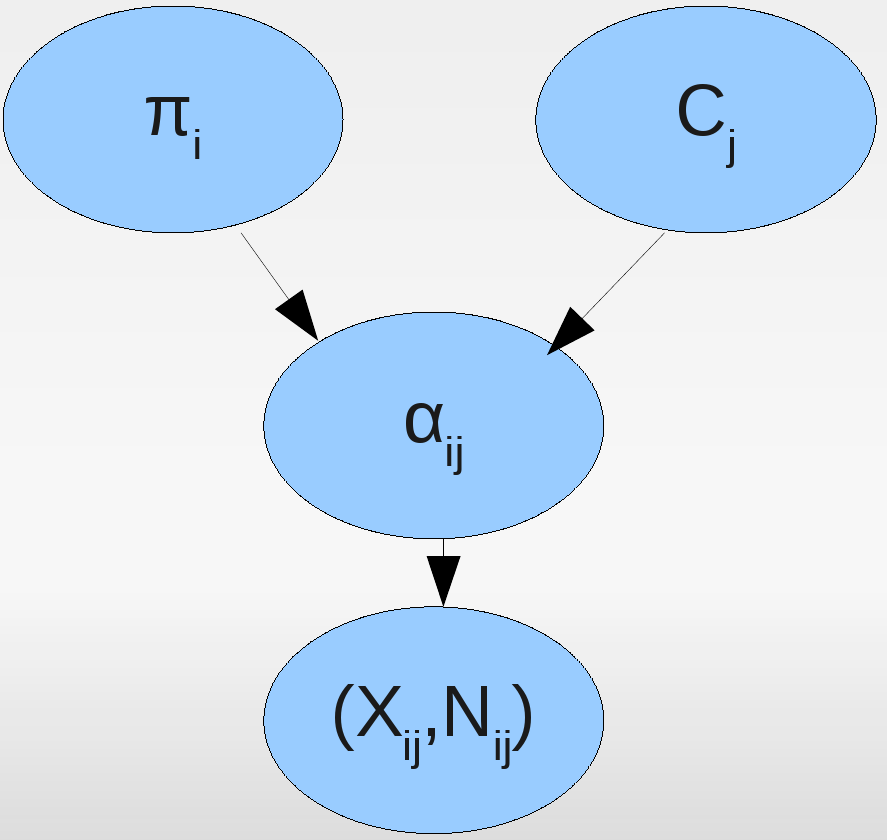
\includegraphics[width=0.2\textwidth]{nicholson-model}
 $\alpha^t = P(\alpha|c^{t-1},\pi^{t-1},x)$
 $\pi^t = P(\pi|c^{t-1},\alpha^t,a)$
 $c^t = P(c|\pi^t,\alpha^t)$
 Implemented using a Gibbs sampler in a FORTRAN program.
 Run on each simulation, and each subset of loci (all,
  not.all.fixed, none.fixed), independently.
}

\subsection{PPP-value calculation}

\section{Results}


Loci fixation?

 Some alleles can be fixed at the end of the simulation,
  $\aij\in\{0,1\}$
 Since we are modeling Single Nucleotide Polymorphisms the data
  are probably not fixed.
 We can consider non-fixed loci only, for the model fitting
  later.
 Criteria:
\begin{description}
\item[not.all.fixed] Throw out the locus if all subpopulations fixed.
\item[none.fixed] Throw out the locus if one or more subpopulations fixed.
\end{description}


\subsection{Simulation verification}

\fig[0.5]{beta}{Distribution of ancestral allele frequencies in our
  simulations follow a truncated $\beta(0.7,0.7)$ distribution.}

\fig{loci-over-time}{Allele frequency evolution of 6 loci in 12
  populations over 100 generations.}

\fig[0.5]{fixation-selection}{foo}

\fig{sim-summary-plot}{foo}

To visualize the influence of the number of generations on each of
these diagnostic plots, we used to the animation
package\cite{animation} to create a series of plots, one for each
generation. These images are put together and viewed in sequence to
form a statistical animation that reveals the dependence on the number
of generations. The animations can be viewed on the accompanying
website:

 \url{http://nicholsonppp.r-forge.r-project.org/}

\subsection{Model estimates}

\fig{anc-est-plot}{To diagnose dependence of model fit on selection
  state, we plot ancestral allele frequency estimates for each loci
  versus actual values from the simulation. Neutral loci are well
  estimated by the model, but loci under balancing and positive
  selection are not well estimated.}

\fig{2009-08-27-notbeta}{Scatter plot matrix for various values of
  ancestral allele frequency $\pi$ for a simulated data set (actual
  simulated values indicated by row/column simulated). Models using
  priors that follow a $\beta(1,1)$ (indicated by fortranr1 and
  winbugs1) and $\beta(0.7,0.7)$ (fortran.old, fortranr0.7, and
  winbugs0.7) were fit using WinBUGS and our FORTRAN program. For
  alleles under positive selection, there are small discrepancies
  between the FORTRAN and WinBUGS programs.}

\fig[0.5]{c-over-time-all}{foo} \fig[0.5]{c-over-time-diff}{foo}
\fig[0.5]{c-over-time-same}{foo} \fig[0.8]{cutoff-plot-few}{foo}

\subsection{Sensitivity of the PPP-value classifier}

\fig[0.8]{dens-several-s-few}{foo} 
\fig[0.8]{dens-several-s-neu}{foo}

\fig[0.8]{cutoff-plot-neu}{foo}
\fig[0.8]{cutoff-plot}{foo}
\fig[0.8]{dens-several-s}{foo}
\fig{fixation-endpoints}{foo}
\fig{gen-pop-dens}{foo}
\fig{gen-pop}{foo}
%\fig{gen-pop-roc}{foo}
%\fig{roc-desc}{foo}
%\fig[0.8]{roc-s}{foo}

\section{Conclusions}

\end{document}
